
\subsection{Error Bars}
\label{sec:errorbars}
{%
\def\pgfplotserror#1{\ensuremath{\epsilon_{#1}}}%
\PGFPlots\ supports error bars for normal and logarithmic plots. 

Error bars are enabled for each plot separately, using \meta{options} after |\addplot|:
\pgfmanualpdflabel{/pgfplots/error bars}{}%
\begin{codeexample}[code only]
\addplot+[error bars/.cd,x dir=both,y dir=both] ...
\end{codeexample}
Error bars inherit all drawing options of the associated plot, but they use their own marker and style arguments additionally.

\begin{codeexample}[]
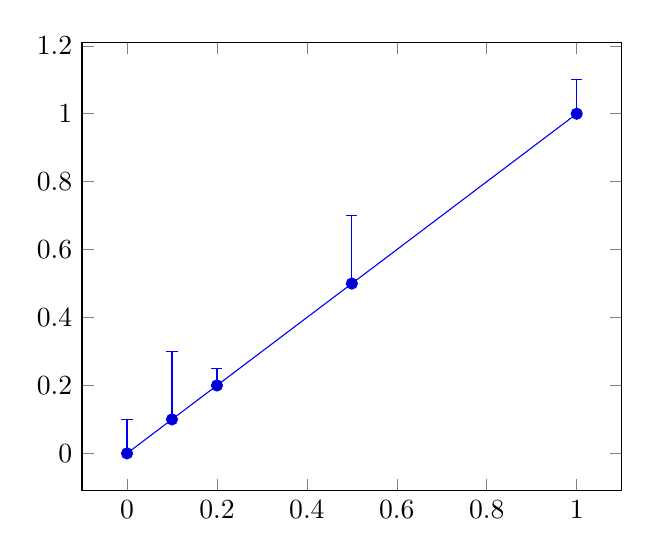
\begin{tikzpicture}
\begin{axis}
\addplot+[error bars/.cd,
	y dir=plus,y explicit]
coordinates {
	(0,0)     +- (0.5,0.1) 
	(0.1,0.1) +- (0.05,0.2)
	(0.2,0.2) +- (0,0.05)
	(0.5,0.5) +- (0.1,0.2)
	(1,1)     +- (0.3,0.1)};
\end{axis}
\end{tikzpicture}
\end{codeexample}

\begin{codeexample}[]
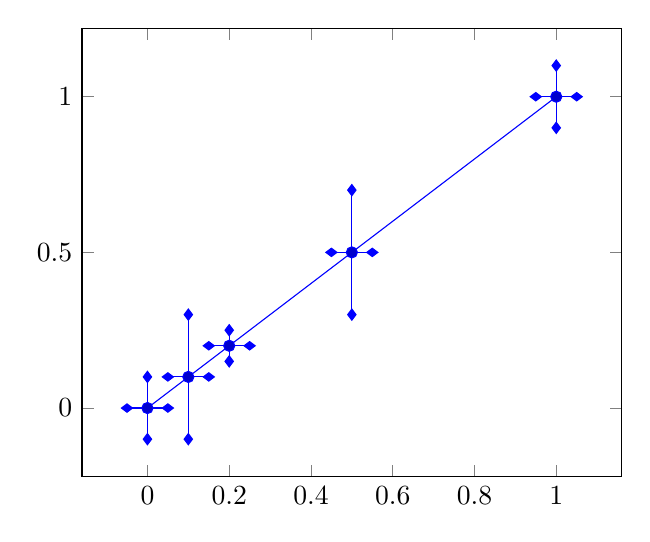
\begin{tikzpicture}
\begin{axis}
\addplot+[error bars/.cd,
	y dir=both,y explicit,
	x dir=both,x fixed=0.05,
	error mark=diamond*]
coordinates {
	(0,0)     +- (0.5,0.1) 
	(0.1,0.1) +- (0.05,0.2)
	(0.2,0.2) +- (0,0.05)
	(0.5,0.5) +- (0.1,0.2)
	(1,1)     +- (0.3,0.1)};
\end{axis}
\end{tikzpicture}
\end{codeexample}

\pgfplotsset{anchor=center,/tikz/every picture/.append style={baseline}}
\begin{codeexample}[]
\pgfplotstabletypeset{pgfplots.testtable2.dat}

\begin{tikzpicture}
\begin{loglogaxis}
\addplot+[error bars/.cd,
	x dir=both,x fixed relative=0.5,
	y dir=both,y explicit relative,
	error mark=triangle*]
	table[x=x,y=y,y error=errory] 
	{pgfplots.testtable2.dat};
\end{loglogaxis}
\end{tikzpicture}
\end{codeexample}
%--------------------------------------------------
% coordinates {
% 	(32,32)
% 	(64,64)
% 	(128,128) +- (0,0.3)
% 	(1024,1024) +- (0,0.2)
% 	(32068,32068) +- (0,0.6)
% 	(64000,64000) +- (0,0.6)
% 	(128000,128000) +- (0,0.6)
% };
%-------------------------------------------------- 

\begin{codeexample}[]
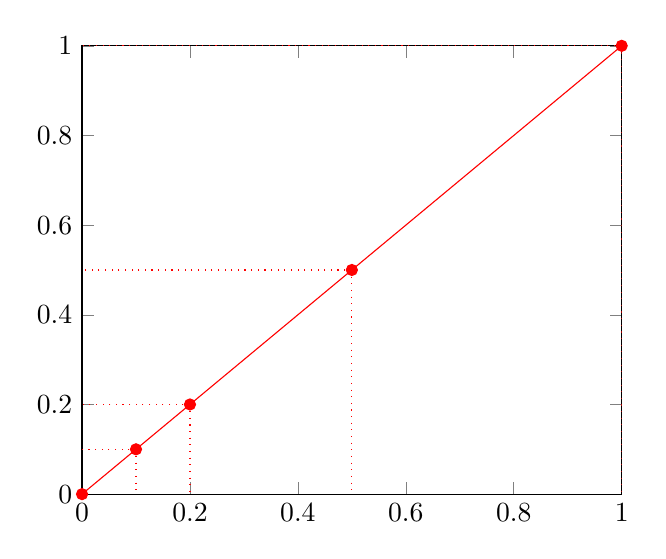
\begin{tikzpicture}
\begin{axis}[enlargelimits=false]
\addplot[red,mark=*] 
	plot[error bars/.cd,
	y dir=minus,y fixed relative=1,
	x dir=minus,x fixed relative=1,
	error mark=none,
	error bar style={dotted}]
coordinates
	{(0,0) (0.1,0.1) (0.2,0.2) 	
	 (0.5,0.5) (1,1)};
\end{axis}
\end{tikzpicture}
\end{codeexample}

\begin{pgfplotsxykey}{error bars/\x\ dir=\mchoice{none,plus,minus,both} (initially none)}
Draws either no error bars at all, only marks at $x+\pgfplotserror x$, only marks at $x-\pgfplotserror x$ or marks at both, $x+\pgfplotserror x$ and $x-\pgfplotserror x$. The $x$-error $\pgfplotserror x$ is acquired using one of the following options.

The same holds for the |y dir| option.
\end{pgfplotsxykey}

\begin{pgfplotsxykey}{error bars/\x\ fixed=\marg{value} (initially 0)}
Provides a common, absolute error $\pgfplotserror x=\text{\meta{value}}$ for all input coordinates.

For linear $x$~axes, the error mark is drawn at $x \pm \pgfplotserror x$ while for logarithmic $x$~axes, it is drawn at $\log( x \pm \pgfplotserror x)$. Computations are performed in \PGF's floating point arithmetics.
\end{pgfplotsxykey}

\begin{pgfplotsxykey}{error bars/\x\ fixed relative=\marg{percent} (initially 0)}
Provides a common, relative error $\pgfplotserror x = \text{\meta{percent}} \cdot x$ for all input coordinates. The argument \meta{percent} is thus given relatively to input $x$ coordinates such that $\text{\meta{percent}} = 1$ means $100\%$.

Error marks are thus placed at $x \cdot (1 \pm \pgfplotserror x)$ for linear axes and at $\log(x \cdot (1 \pm \pgfplotserror x))$ for logarithmic axes. Computations are performed in floating point for linear axis and using the identity $\log(x \cdot (1 \pm \pgfplotserror x)) = \log(x) + \log( 1 \pm \pgfplotserror x)$ for logarithmic scales.
\end{pgfplotsxykey}

\begin{pgfplotsxykey}{error bars/\x\ explicit}
Configures the error bar algorithm to draw $x$-error bars at any input coordinate for which user-specified errors are available.
 Each error is interpreted as absolute error, see |x fixed| for details.

The different input formats of errors are described in section~\ref{sec:errorbar:input}.
\end{pgfplotsxykey}

\begin{pgfplotsxykey}{error bars/\x\ explicit relative}
Configures the error bar algorithm to draw $x$-error bars at any input coordinate for which user-specified errors are available.
 Each error is interpreted as relative error, that means error marks are placed at $x (1 \pm \text{\meta{value}}(x))$ (works as for |error bars/x fixed relative|).
\end{pgfplotsxykey}


\begin{pgfplotskey}{error bars/error mark=\meta{marker}}
Sets an error marker for any error bar. \marg{marker} is expected to be a valid plot mark, see section~\ref{sec:markers}.
\end{pgfplotskey}

\begin{pgfplotskey}{error bars/error mark options=\marg{key-value-list}}
Sets a key-value list of options for any error mark. This option works similary to the \Tikz\ `|mark options|' key.
\end{pgfplotskey}

\begin{pgfplotskey}{error bars/error bar style=\marg{key-value-list}}
Appends the argument to `|/pgfplots/every error bar|' which is installed at the beginning of every error bar.
\end{pgfplotskey}

\begin{pgfplotscodetwokey}{error bars/draw error bar}
Allows to change the default drawing commands for error bars. The two arguments are
\begin{itemize} 
\item the source point, $(x,y)$ and
\item the target point, $(\tilde x,\tilde y)$.
\end{itemize}
Both are determined by \PGFPlots\ according to the options described above. The default code is
\begin{codeexample}[code only]
\pgfplotsset{
	/pgfplots/error bars/draw error bar/.code 2 args={%
		\pgfkeysgetvalue{/pgfplots/error bars/error mark}%
			{\pgfplotserrorbarsmark}%
		\pgfkeysgetvalue{/pgfplots/error bars/error mark options}%
			{\pgfplotserrorbarsmarkopts}%
		\draw #1 -- #2 node[pos=1,sloped,allow upside down] {%
			\expandafter\tikz\expandafter[\pgfplotserrorbarsmarkopts]{%
				\expandafter\pgfuseplotmark\expandafter{\pgfplotserrorbarsmark}%
				\pgfusepath{stroke}}%
		};
	}
}
\end{codeexample}
\end{pgfplotscodetwokey}

\subsubsection{Input Formats of Error Coordinates}
\label{sec:errorbar:input}%
Error bars with explicit error estimations for single data points require some sort of input format. This applies to `|error bars/|\meta{[xy]}| explicit|' and `|error bars/|\meta{[xy]}| explicit relative|'.

Error bar coordinates can be read from `|plot coordinates|' or from `|plot table|'. The inline plot coordinates format is
\begin{codeexample}[code only]
\addplot coordinates {
	(1,2) +- (0.4,0.2)
	(2,4) +- (1,0)
	(3,5)
	(4,6) +- (0.3,0.001)
}
\end{codeexample}
where $(1,2) \pm (0.4,0.2)$ is the first coordinate, $(2,4) \pm (1,0)$ the second and so forth. The point $(3,5)$ has no error coordinate.

The `|plot table|' format is
\begin{codeexample}[code only]
\addplot table[x error=COLNAME,y error=COLNAME]
\end{codeexample}
or
\begin{codeexample}[code only]
\addplot table[x error index=COLINDEX,y error index=COLINDEX]
\end{codeexample}
These options are used as the `|x|' and `|x index|' options.

You can supply error coordinates even if they are not used at all; they will be ignored silently in this case.

}%
